%
% chapter.tex -- Graphenbeschreibung mit Matrizen
%
% (c) 2020 Prof Dr Andreas Müller, Hochschule Rapperswil
%
\chapter{Graphen
\label{buch:chapter:graphen}}
\lhead{Graphen}
\rhead{}
Ein Graph ist eine Menge von Knoten, die untereinander mit Kanten
verbunden sind.
Graphen können zum Beispiel verwendet werden um Netzwerke zu beschreiben,
aber auch viele andere Datenstrukturen.
\index{Graph}%
Die Knoten können einzelne Objekte beschreiben, die Kanten beschreiben
dann Beziehungen zwischen diesen Objekten.
Graphen haben zwar nur eine eindimensionale Geometrie, sie können aber auch als
erste Approximation dreidimensionaler Objekte dienen.

Die Bedeutung des Graphenkozeptes wird unterstrichen von der Vielzahl
von Fragestellungen, die über Graphen gestellt, und der
zugehöriten Lösungsalgorithmen, die zu ihrer Beantwortung gefunden
worden sind.
Die Komplexitätstheorie hat sogar gezeigt, dass sich jedes diskrete
Problem in ein Graphenproblem umformulieren lässt.
\index{Komplexitätstheorie}%

Das Problem, einen Stundenplan zu finden, der sicherstellt, dass
alle Studierenden jedes Fach besuchen können, für die sie sich
angemeldet haben, lässt sich zum Beispiel wie folgt als ein
Graphenproblem formulieren.
Die Fächer betrachten wir als Knoten des Graphen.
Für jedes Paar von Fächern ziehen wir eine Kante des Graphen, wenn 
sich mindestens ein Studierender für beide Fächer angemeldet hat.
Die Kante drückt aus, dass die beiden Fächer nicht zur gleichen Zeit
geplant werden dürfen.
Das Problem, einen Stundenplan zu finden, besteht jetzt darin, für
jedes Fach ein Zeitintervall zu finden, während dem es durchgeführt
werden soll.
\index{Stundenplan}%
Natürlich steht nur eine beschränkte Anzahl Zeitintervalle zur Verfügung
und benachbarte Knoten dürfen nicht ins gleiche Zeitintervall geplant
werden.
Das zugehörige abstrakte Graphenproblem heisst das Färbeproblem: 
\index{Färbeproblem}%
ist es möglich, mit einer beschränkten Anzahl von Farben die Knoten
des Graphen so einzufärben, dass benachbarte Knoten niemals die gleiche
Farbe haben.

In diesem Kapitel soll zunächst gezeigt werden, wie man Graphen mit 
Hilfe von Matrizen beschreiben kann
(Abschnitt~\ref{buch:section:beschreibung-von-graphen-mit-matrizen}).
Das Ziel dabei ist natürlich, die Hilfsmittel der Matrixalgebra
zur Lösung von Graphenprobleme hinzuzuziehen.
Die spektrale Graphentheorie in
Abschnitt~\ref{buch:section:spektrale-graphentheorie} verwendet
die Eigenwerte und Eigenvektoren der zugehörigen Matrix, um Aussagen
über den Graphen zu machen.
\index{Graphentheorie!spektrale}%
In Abschnitt~\ref{buch:section:wavelets-auf-graphen} wird gezeigt,
wie spektralen Eigenschaften verwendet werden können, um eine
Art von Wavelets auf einem Graphen zu definieren.
Damit ensteht eine für gewisse Anwendungen besonders leistungsfähige
Basis zur Beschreibung von Funktionen auf dem Graphen.

%
% beschreibung.tex -- Beschreibung von Graphen mit Matrizen
%
% (c) 2020 Prof Dr Andreas Müller, Hochschule Rapperswil
%
\section{Beschreibung von Graphen mit Matrizen
\label{buch:section:beschreibung-von-graphen-mit-matrizen}}
\rhead{Beschreibung mit Matrizen}
Als universelles kombinatorisches Modell sind Graphen für eine
Vielzahl von Problemlösungen interessant.
Zum Beispiel zeigt Kapitel~\ref{chapter:munkres}, wie man
ein Zuordnungsproblem als Graphenproblem formulieren kann.
Die Lösung erfolgt dann allerdings zweckmässigerweise unter
Verwendung einer Matrix.
Ziel dieses Abschnitts ist, Graphen und ihre zugehörigen Matrizen
zu definieren und erste Eigenschaften des Graphen mit algebraischen
Mitteln abzuleiten.
Die Präsentation ist allerdings nur ein erster Einstieg, tiefer
gehende Information kann in \cite{skript:brualdi} gefunden werden.

\subsection{Ungerichtete und gerichtete Graphen
\label{subsection:definition-von-graphen}}
In der Einleitung wurde bereits eine informelle
Beschreibung des Konzeptes eines Graphen gegeben.
Um zu einer Beschreibung mit Hilfe von Matrizen zu kommen,
wird eine exakte Definition benötigt.
Dabei werden sich einige Feinheiten zeigen, die für Anwendungen wichtig
sind und sich in Unterschieden in der Definition der zugehörigen Matrix 
äussern.

\subsubsection{Ungerichtete Graphen}
Die Grundlage für alle Arten von Graphen ist eine Menge $V$ von {\em Knoten},
auch {\em Vertizes} genannt.
\index{Knoten}%
\index{Vertex}%
Die Unterschiede zeigen sich in der Art und Weise, wie die Knoten
mit sogenannten Kanten
\index{Kante}%
verbunden werden.
Bei einem ungerichteten Graphen sind die beiden Endpunkte einer Kante
gleichwertig, es gibt keine bevorzugte Reihenfolge oder Richtung der
Kante.
Eine Kante ist daher vollständig spezifiziert, wenn wir die
Menge der Endpunkte kennen.
Dies führt auf die folgende Definition eines ungerichteten Graphen.

\begin{definition}
\label{buch:def:ungerichteter-graph}
\index{Graph!ungerichteter}%
\index{ungerichteter Graph}%
Ein {\em ungerichteter Graph} ist eine endliche Menge $V$ von {\em Knoten}
und eine Menge $E$ von zweielementigen Teilmengen 
\[
E \subset \{\, \{a,b\}\subset V\,|\, a\ne b\}.
\]
Die Elemente von $E$ heissen {\em Kanten} (edges).
\end{definition}

Man beachte, dass es keine Kante gibt, die einen Knoten $a\in V$
mit sich selbst verbindet, da die zugehörige Menge $\{a,a\}=\{a\}$
nicht aus zwei verschiedenen Elementen besteht, wie die
Definition~\ref{buch:def:ungerichteter-graph} dies verlangt.
Es gibt also keine Schleifen an einem Knoten.

\begin{beispiel}
Ein elektrisches Netzwerk von ohmschen Widerständen kann mit Hilfe
eines ungerichteten Graphen beschrieben werden.
Ohmsche Widerstände hängen nicht von der Richtung des Stromflusses
durch die Widerstände ab.
Will man Spannungen und Ströme in einem solchen Netzwerk berechnen,
ist auch das Fehlen von Schleifen, die von $a$ zu $a$ führen, kein
Verlust.
Die Endpunkte solcher Widerstände wären immer auf dem gleichen Potential.
Folglich würde kein Strom fliessen und sie hätten keinen Einfluss auf
das Verhalten des Netzwerkes.
Sie können einfach weggelassen werden.
\end{beispiel}

\subsubsection{Gerichtete Graphen}
In vielen Anwendungen sind die Endpunkte einer Kante nicht austauschbar.
In einem Strassennetz sind Einbahnstrassen nicht in beiden Richtungen
befahrbar.
Anfangs- und Endpunkt einer Kante müssen in einem solche Graphen
unterschieden werden.
Eine zweielementige Menge ist daher nicht mehr eine geeignete Abstraktion
für die Kante, ein (geordnetes) Paar von Vertizes passt besser.

\begin{definition}
\label{buch:def:gerichteter-graph}
\index{Graph!gerichteter}%
\index{gerichteter Graph}%
Ein {\em gerichteter Graph} ist eine endliche Menge $V$ von Knoten
und eine Menge $E \subset V\times V$ von gerichteten Kanten.
Ausserdem gibt es zwei Abbildungen
\[
\begin{aligned}
a&\colon E\to V: (p,q) \mapsto a((p,q)) = p
\\
e&\colon E\to V: (p,q) \mapsto e((p,q)) = q.
\end{aligned}
\]
Der Knoten $a(k)$ heisst der {\em Anfangspunkt} der Kante $k\in E$,
$e(k)$ heisst der {\em Endpunkt}.
\end{definition}

In einem gerichteten Graphen gehört also zu jeder Kante auch eine Richtung.
Die Unterscheidung von Anfangs- und Endpunkt einer Kante ist sinnvoll
geworden.
Ausderdem ist eine Kante $(a,a)$ wohldefiniert, also eine Kante, die vom
Knoten $a$ wieder zu $a$ zurück führt.

Man kann einen ungerichteten Graphen in einen gerichteten Graphen
verwandeln, indem jede Kante $\{u,v\}$ durch zwei Kanten 
$(u,v)$ und $(v,u)$ ersetzt wird.
Aus dem ungerichteten Graphen $(V,E)$ mit Knotenmenge $V$ und Kantenmenge
$E$ wird so der gerichtete Graph
$(V,E')$ mit der Kantenmenge
\begin{equation*}
E' 
=
\{
(u,v)
\,|\,
\{u,v\}\in E
\}.
\end{equation*}
Eine umgekehrte Zuordnung eines gerichteten zu einem ungerichteten
Graphen ist nicht möglich, da eine ``Schleife'' $(v,v)$ nicht in eine Kante
des ungerichteten Graphen abgebildet werden kann.

In einem gerichteten Graphen kann man sinnvoll von gerichteten Pfaden
sprechen.
\index{Pfad}%
Ein {\em Pfad} $\gamma$ in einem gerichteten Graphen $(V,E)$ ist eine Folge
$k_1,\dots,k_r\in E$ von Kanten derart, dass $e(k_i) = a(k_{i+1})$
für $i=1,\dots,r-1$.
Dies bedeutet, dass der Endpunkt jeder Kante mit dem Anfangspunkt der
nachfolgenden Kante übereinstimmt.
Die {\em Länge} des Pfades $\gamma=(k_1,\dots,k_r)$ ist $|\gamma|=r$.

\subsection{Adjazenzmatrix}
\begin{figure}
\centering
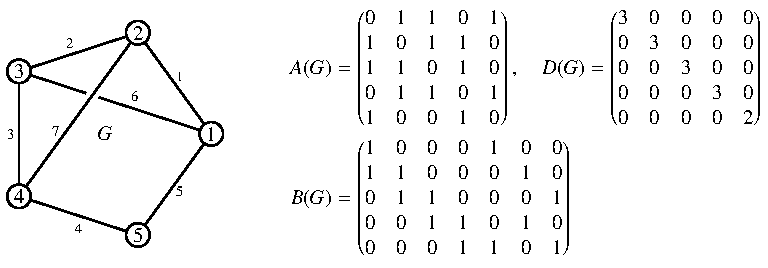
\includegraphics{chapters/70-graphen/images/adjazenzu.pdf}
\caption{Adjazenz-, Inzidenz- und Gradmatrix eines ungerichteten
Graphen mit fünf Knoten und sieben Kanten.
\label{buch:graphen:fig:adjazenzu}}
\end{figure}
Eine naheliegende Beschreibung eines Graphen mit Hilfe einer
Matrix kann man wie folgt erhalten.
Zunächst werden die Knoten aus der Menge $V$ durch die Zahlen
$1,\dots,n$ mit $n=|V|$ ersetzt.
Diese Zahlen werden dann als Zeilen- uns Spaltenindizes interpretiert.
Die zum Graphen gehörige sogenannte {\em Adjazenzmatrix} $A(G)$
enthält die Einträge
\begin{equation}
a_{i\!j}
=
\begin{cases}
1&\qquad  \{j,i\} \in E\\
0&\qquad  \text{sonst.}
\end{cases}
\label{buch:graphen:eqn:adjazenzmatrix}
\end{equation}
Die Matrix hat also genau dann einen von Null verschiedenen Eintrag
in Zeile $i$ und Spalte $j$, wenn die beiden Knoten $i$ und $j$
im Graphen verbunden sind.
Die Adjazenzmatrix eines ungerichteten Graphen ist immer symmetrisch.
Ein Beispiel ist in Abbildung~\ref{buch:graphen:fig:adjazenzu}
dargestellt.

\begin{figure}
\centering
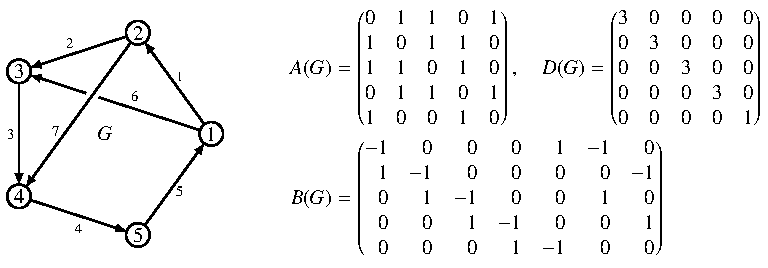
\includegraphics{chapters/70-graphen/images/adjazenzd.pdf}
\caption{Adjazenz-, Inzidenz- und Gradmatrix eines gerichteten
Graphen mit fünf Knoten und sieben Kanten.
Die roten Einträge in der Adjazenzmatrix $A(G)$ heben die
Unterschiede zur Adjazenzmatrix des gerichteten Graphen
von Abbildung~\ref{buch:graphen:fig:adjazenzu} hervor.
\label{buch:graphen:fig:adjazenzd}}
\end{figure}
Die Adjazenzmatrix kann auch für einen gerichteten Graphen definiert
werden wie dies in in Abbildung~\ref{buch:graphen:fig:adjazenzd}
illustriert ist.
Ihre Einträge sind in diesem Fall definiert mit Hilfe der 
gerichteten Kanten als
\begin{equation}
A(G)_{i\!j}
=
a_{i\!j}
=
\begin{cases}
1&\qquad  (j,i) \in E\\
0&\qquad  \text{sonst.}
\end{cases}
\label{buch:graphen:eqn:adjazenzmatrixgerichtet}
\end{equation}
Die Matrix $A(G)$ hat also genau dann einen nicht verschwindenden
Matrixeintrag in Zeile $i$ und Spalte $j$, wenn es eine Verbindung
von Knoten $j$ zu Knoten $i$ gibt.

\subsubsection{Adjazenzmatrix und die Anzahl der Pfade}
Die Beschreibung des Graphen mit der Adjazenzmatrix $A=A(G)$ nach
\eqref{buch:graphen:eqn:adjazenzmatrix} ermöglicht bereits, eine
interessante Aufgabe zu lösen.

\begin{satz}
\label{buch:graphen:pfade-der-laenge-n}
Der gerichtete Graph $G=([n],E)$ werde beschrieben durch die Adjazenzmatrix
$A=A(G)$.
Dann gibt das Element $(A^n)_{ji}$ in Zeile $j$ und Spalte $i$ von $A^n$
die Anzahl der Wege der Länge $n$ an, die von Knoten $i$ zu Knoten $j$ führen.
Insbesondere kann man die Definition~\eqref{buch:graphen:eqn:adjazenzmatrix}
formulieren als: In Zeile $j$ und Spalte $i$ der Matrix steht die Anzahl
der Pfade der Länge $1$, die $i$ mit $j$ verbinden.
\end{satz}
\index{Anzahl der Pfade}%

\begin{proof}[Beweis]
Zur Unterscheidung der Matrix der Wegzahlen von $A^n$ schreiben wir
$A^{(n)}$ für die Matrix, die in Zeile
$j$ und Spalte $i$ die Anzahl der Pfade der Länge $n$ von $i$ nach $j$
enhält.
Die zugehörigen Matrixelemente schreiben wir $a_{ji}^{n}$ bzw.~$a_{ji}^{(n)}$.
Wir haben also zu zeigen, dass $A^n = A^{(n)}$.

Wir beweisen mit Hilfe von vollständiger Induktion,
dass $A^n$ Pfade der Länge $n$ zählt.
Es ist klar, dass $A^1$ die genannte Eigenschaft hat.
Der Fall $A^1$ dient daher als Induktionsverankerung.

Wir nehmen daher im Sinne einer Induktionsannahme an, dass bereits
bewiesen ist, dass das Element in Zeile
$j$ und Spalte $i$ von $A^{n-1}$ die Anzahl der Pfade der Länge $n-1$
zählt, dass also $A^{n-1}=A^{(n-1)}$.
%Dies ist die Induktionsannahme.

Wir bilden jetzt alle Pfade der Länge $n$ von $i$ nach $k$.
Ein Pfad der Länge besteht aus einem Pfad der Länge $n-1$, der von $i$ zu
einem beliebigen Knoten $j$ führt, gefolgt von einer einzelnen Kante,
die von $j$ nach $k$ führt.
Ob es eine solche Kante gibt, zeigt das Matrixelement $a_{k\!j}$ an.
Das Element in Zeile $j$ und Spalte $i$ der Matrix $A^{(n-1)}$ gibt
die Anzahl der Wege von $i$ nach $j$ an.
Es gibt also $a_{k\!j}\cdot a_{ji}^{(n-1)}$ Wege der Länge $n$, die von $i$
nach $k$ führen, aber als zweitletzten Knoten über den Knoten $j$ führen.
Die Gesamtzahl der Wege der Länge $n$ von $i$ nach $k$ ist daher
\[
a_{ki}^{(n)}
=
\sum_{j=1}^n a_{k\!j} a_{ji}^{(n-1)}.
\]
In Matrixschreibweise bedeutet dies
\[
A^{(n)}
=
A\cdot A^{(n-1)}
=
A\cdot A^{n-1}
=
A^n.
\]
Beim zweiten Gleichheitszeichen haben wir die Induktionsannahme
verwendet.
Damit ist der Induktionsschritt vollzogen und der Satz bewiesen.
\end{proof}

Speziell geben die Diagonalelemente von $A^n$ die Zahl der geschlossenen
Pfade an.
$(A^n)_{ii}$ ist die Anzahl der geschlossenen Pfade, die $i$ enthalten.

Der Satz~\ref{buch:graphen:pfade-der-laenge-n} ermöglicht auch, einen 
Algorithmus für den sogenannten Durchmesser eines Graphen zu formulieren.

\begin{definition}
\index{Durchmesser eines Graphen}%
\index{Graph!Durchmesser des}%
Der {\em Durchmesser} eines Graphen ist die kürzeste Länge $d$ derart, dass
es zwischen zwei beliebigen Knoten einen Pfad der Länge $\le d$ gibt.
\end{definition}

Der Durchmesser $d$ eines Graphen ist der kleinste Exponent derart,
dass $A^d$ keine ausserdiagonalen Einträge $0$ hat.
Die Diagonalelemente von $A^n$ zählen die Anzahl der geschlossenen Pfade
der Länge $n$, die durch einen Knoten führen.
Diese können für den Durchmesser ignoriert werden.
Man kann also Potenzen $A^n$ berechnen bis keine Einträge $0$ mehr vorhanden
sind.

\begin{beispiel}
\begin{figure}
\centering
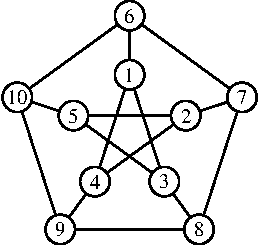
\includegraphics{chapters/70-graphen/images/peterson.pdf}
\caption{Peterson-Graph mit zehn Knoten.
\label{buch:figure:peterson}}
\end{figure}
Der Peterson-Graph von Abbildung~\ref{buch:figure:peterson}
hat die Adjazenzmatrix
\[
G
=
\begin{pmatrix}
%1  2  3  4  5  6  7  8  9 10
 0& 0& 1& 1& 0& 1& 0& 0& 0& 0\\ %  1
 0& 0& 0& 1& 1& 0& 1& 0& 0& 0\\ %  2
 1& 0& 0& 0& 1& 0& 0& 1& 0& 0\\ %  3
 1& 1& 0& 0& 0& 0& 0& 0& 1& 0\\ %  4
 0& 1& 1& 0& 0& 0& 0& 0& 0& 1\\ %  5
 1& 0& 0& 0& 0& 0& 1& 0& 0& 1\\ %  6
 0& 1& 0& 0& 0& 1& 0& 1& 0& 0\\ %  7
 0& 0& 1& 0& 0& 0& 1& 0& 1& 0\\ %  8
 0& 0& 0& 1& 0& 0& 0& 1& 0& 1\\ %  9
 0& 0& 0& 0& 1& 1& 0& 0& 1& 0   % 10
\end{pmatrix}.
\]
Durch Nachrechnen kann man bestätigen, dass $G^3$ keine
Ausserdiagonalelemente $0$ enthält:
\[
G^3
=
\begin{pmatrix}
 0& 2& 5& 5& 2& 5& 2& 2& 2& 2\\
 2& 0& 2& 5& 5& 2& 5& 2& 2& 2\\
 5& 2& 0& 2& 5& 2& 2& 5& 2& 2\\
 5& 5& 2& 0& 2& 2& 2& 2& 5& 2\\
 2& 5& 5& 2& 0& 2& 2& 2& 2& 5\\
 5& 2& 2& 2& 2& 0& 5& 2& 2& 5\\
 2& 5& 2& 2& 2& 5& 0& 5& 2& 2\\
 2& 2& 5& 2& 2& 2& 5& 0& 5& 2\\
 2& 2& 2& 5& 2& 2& 2& 5& 0& 5\\
 2& 2& 2& 2& 5& 5& 2& 2& 5& 0
\end{pmatrix}
=
2(U-I) + 3G.
\]
Daraus kann man jetzt ablesen, dass der Durchmesser des Petersongraphen
$d=3$ ist.
Man kann aber noch mehr ablesen:
\begin{itemize}
\item
Es gibt keine geschlossenen Pfade der Länge $3$.
\item
Zwischen benachbarten Knoten gibt es jeweils $5$ Pfade der Länge $3$,
zwischen nicht benachbarten Knoten gibt es genau $2$ Pfade der Länge $3$.
\qedhere
\end{itemize}
\end{beispiel}

Das Beispiel illustriert, wie sich Zählaufgaben von Pfaden leicht mit dem
Matrizenprodukt erledigen lassen.
Trotzdem ist der Algorithmus nicht unbedingt effizient, da der Aufwand
zur Berechnung des Matrizenproduktes relativ gross sein kann.
Für den Peterson-Graphen können die gefundenen Aussagen über die Anzahl
von Pfaden durch Ausnützung der Symmetrien des Graphen leichter direkt
gefunden werden.


\subsection{Inzidenzmatrix
\label{buch:graphen:subsection:inzidenzmatrix}}
Die Adjazenzmatrix kann zusätzliche Information, die möglicherweise
mit den Kanten verbunden ist, nicht mehr darstellen.
Dies tritt zum Beispiel in der Informatik bei der Beschreibung
endlicher Automaten auf, wo zu jeder gerichteten Kante auch noch
Buchstaben gehören, für die der Übergang entlang dieser Kante
möglich ist.
Oder in der Elektrotechnik, wo jedes Bauteil in einem elektrischen
Netzwerk eine Impedanz hat.

\subsubsection{Beschriftete Graphen}
Ein beschrifteter Graph löst dieses Problem.

\begin{definition}
Eine {\em Beschriftung}
eines gerichteten oder ungerichteten Graphen $G=(V,E)$ 
mit Elementen der Menge $L$, den Labels,
ist eine Abbildung $l\colon E\to L$.
\index{Beschriftung}%
\end{definition}

Einen gerichteten, beschrifteten Graphen können wir 
statt mit einer Beschriftungsabbildung $l$ auch dadurch erhalten,
dass wir Kanten als Tripel betrachten, die ausser den Knoten auch
noch den Wert der Beschriftung enthalten.

\begin{definition}
\label{buch:graphen:def:beschriftetergraphgerichtet}
Ein gerichteter Graph mit beschrifteten Kanten ist eine Menge $V$ von 
Knoten und eine Menge von beschrifteten Kanten der Form
\[
E \{ (u,v,l)\in V^2\times L \mid \text{Eine Kante mit Beschriftung $l$ führt von $u$ nach $v$}\}.
\]
Die Menge $L$ enthält die möglichen Beschriftungen der Kanten.
\end{definition}

Diese Definition gestattet, dass zwischen zwei Knoten $u$ und $v$
mehrere Kanten vorhanden sind, die sich durch die Beschriftung
unterscheiden.

\subsubsection{Inzidenzmatrix}
Die Adjazenzmatrix bildet nur die Nachbarschaftsbeziehung ab,
sie sagt nichts aus über die ``Qualität'' der Verbindung, die durch
die Beschriftung einer Kante angezeigt wird.
Nach Definition~\ref{buch:graphen:def:beschriftetergraphgerichtet}
ist es auch möglich, dass mehrere Kanten von $a$ nach $e$ führen,
die Adjazenzmatrix kann diese ebenfalls nicht unterscheiden.
Die {\em Inzidenzmatrix}
löst dieses Problem.
\index{Inzidenzmatrix}%
Dazu werden zunächst zusätzlich die Kanten $1,\dots,m$
numeriert, wobei Kanten mit verschiedenen Beschriftungen separat
gezählt werden.
Die Matrixeinträge
\[
b_{i\!j} = \begin{cases}
1\qquad&\text{Knoten $i$ ist ein Endpunkt von Kante $j$}
\\
0\qquad&\text{sonst}
\end{cases}
\]
der Inzidenzmatrix $B(G)$
stellen die Beziehung zwischen Kanten und Knoten her.
Für einen gerichteten Graphen wird in der Inzidenzmatrix für
den Anfangspunkt einer Kante $-1$ eingetragen und für den
Endpunkt $+1$.
Die Inzidenzmatrizen $B(G)$ für die Graphen der beiden Beispiele
in den Abbildungen~\ref{buch:graphen:fig:adjazenzu} und
\ref{buch:graphen:fig:adjazenzd} ist ebendort angegeben.

\subsubsection{Inzidenzmatrix und Adjazenzmatrix}
Sei $B(G)$ die Inzidenzmatrix eines ungerichteten Graphen $G$. 
Die Spalten von $B(G)$ sind mit den Kanten des Graphen indiziert.
Die Matrix $B(G)B(G)^t$ ist eine quadratische Matrix, deren
Zeilen und Spalten mit den Knoten des Graphen indiziert sind.
In dieser Matrix geht die Information über die individuellen
Kanten wieder verloren.
Sie hat für $i\ne j$ die Einträge
\begin{align*}
(B(G)B(G)^t)_{i\!j}
&=
\sum_{\text{$k$ Kante}} b_{ik}b_{jk}
\\
&=\text{Anzahl der Kanten, die $i$ mit $j$ verbinden}
\\
&=a_{i\!j}.
\end{align*}
Die Adjazenzmatrix eines Graphen lässt sich also aus der
Inzidenzmatrix berechnen.

\subsubsection{Gradmatrix}
\index{Gradmatrix}%
Die Diagonale von $B(G)B(G)^t$ eines ungerichteten Graphen $G$
enthält die Werte
\begin{align}
(B(G)B(G)^t)_{ii}
&=
\sum_{\text{$k$ Kante}} b_{ik}^2
=
\text{Anzahl Kanten, die im Knoten $i$ enden}
\label{buch:graphen:eqn:gradmatrix}
\end{align}
Der {\em Grad} eines Knoten eines Graphen ist die Anzahl der
\index{Grad eines Knotens}%
Kanten, die in diesem Knoten enden.
Die Diagonalmatrix, die aus den Graden der Knoten besteht, heisst die
Gradmatrix $D(G)$ des Graphen.
Es gilt daher $B(G)B(G)^t = A(G) + D(G)$.
Für Beispiele siehe die Abbildungen~\ref{buch:graphen:fig:adjazenzu} und
\ref{buch:graphen:fig:adjazenzd}.

\subsubsection{Gerichtete Graphen}
Für einen gerichteten Graphen ändert sich an der Diagonalen
der Matrix $B(G)B(G)^t$ nichts.
Sei $k$ die Kante, die vom Knoten $j$ zum Knoten $i$ führt.
Die Einträge in der Inzidenzmatrix sind daher $b_{ik}=1$ und $b_{jk}=-1$.
Da es nur eine solche Kante gibt (der Graph ist nicht beschriftet),
ist $b_{ik}b_{jk}$ der einzige Term in der Summe, mit der das
Matrixelement
\begin{equation}
a_{i\!j}
=
(B(G)B(G)^t)_{i\!j}
=
\sum_{\kappa} b_{i\kappa}b_{j\kappa}
=
b_{ik}b_{jk}
=
-1
\label{buch:graphen:eqn:ausserdiagonal}
\end{equation}
berechnet wird.
Für einen gerichteten Graphen sind daher alle Ausserdiagonalelemente
negativ.

\subsubsection{Anwendung: Netlist}
Eine natürliche Anwendung eines gerichteten und beschrifteten Graphen
ist eine elektronische Schaltung.
Die Knoten des Graphen sind untereinander verbundene Leiter, sie werden
auch {\em nets} genannt. 
Die beschrifteten Kanten sind die elektronischen Bauteile, die solche
nets miteinander verbinden.
Die Inzidenzmatrix beschreibt, welche Anschlüsse eines Bauteils mit
welchen nets verbunden werden müssen.
Die Informationen in der Inzidenzmatrix werden also in einer
Applikation zum Schaltungsentwurf in ganz natürlicher Weise erhoben.

\subsection{Die Laplace-Matrix
\label{subsection:laplace-matrix}}
Will man ein elektrisches Netzwerk modellieren oder den Transport
von Wärme durch eine Gitterstruktur berechnen, dann muss man zwar den
Kanten des Netzwerks eine ``Stromrichtung'' geben um ausdrücken zu können,
in welche Richtung der Strom oder die Wärmeenergie fliesst.
Trotzdem gestattet man natürlich auch den Stromfluss in Gegenrichtung.

Wir gehen also aus von einem ungerichteten Graphen $G$, aus dem
wir einen gerichteten Graphen $G'$ machen.
Zu jeder Kante $\{a,b\}$ von $G$ wählen wir genau eine der möglichen
Orientierungen $(a,b)$ oder $(b,a)$ im Graphen $G'$.
Aus der Inzidenzmatrix $B(G')$ lässt sich jetzt ein Operator konstruieren,
der für die Anwendungen besonders gut geeignet ist.

\begin{definition}
\label{buch:graphen:def:laplace-matrix}
Die {\em Laplace-Matrix} des Graphen $G$ ist
\[
L(G) = B(G')B(G')^t,
\]
wobei $G'$ ein wie oben konstruierter gerichteter Graph ist.
\end{definition}

Wir müssen uns davon überzeugen, dass diese Definition sinnvoll ist
und nicht etwa von der Wahl von $G'$ abhängt.
Diese klärt der folgende Satz.

\begin{satz}
Die Laplace-Matrix eines ungerichteten Graphen $G$ ist
\begin{equation}
L(G) = D(G) - A(G)
\label{buch:graphen:eqn:laplace-definition}
\end{equation}
und somit insbesondere unabhängig von der Wahl des Graphen $G'$,
der für die Definition von $L(G)$ verwendet wurde.
\end{satz}

\begin{proof}[Beweis]
Aufgrund der Konstruktion des Graphen $G'$ sind die Diagonalelemente
der Laplace-Matrix
$L(G)=B(G')B(G')^t$ nach \eqref{buch:graphen:eqn:gradmatrix} genau
die Elemente der Gradmatrix $D(G)$.
Die ausserdiagonalen Elemente sind nach
\eqref{buch:graphen:eqn:ausserdiagonal}
genau dann von $0$ verschieden, wenn es in $G$ eine Verbindung zwischen
den beiden Knoten gibt.
Im Produkt $B(G')B(G')^t$ summieren sie sich zu den ausserdiagonalen
Elementen von $-A(G)$.
Damit ist die Formel
\eqref{buch:graphen:eqn:laplace-definition}
nachgewiesen.
\end{proof}

Die Laplace-Matrix tritt zum Beispiel als Diskretisation des Laplace-Operators
in partiellen Differentialgleichungen auf.
Sie ist die Basis für die Untersuchungen der spektralen Graphentheorie
in Abschnitt~\ref{buch:section:spektrale-graphentheorie}.


%
% spektral.tex -- spektrale Graphentheorie
%
% (c) 2020 Prof Dr Andreas Müller, Hochschule Rapperswil
%
\section{Spektrale Graphentheorie
\label{buch:section:spektrale-graphentheorie}}
\rhead{Spektrale Graphentheorie}
Die Adjazenzmatrix, die Gradmatrix und damit natürlich auch
die Laplace-Matrix codieren alle wesentliche Information eines
ungerichteten Graphen.
Sie operiert auf Vektoren, die für jeden Knoten des Graphen eine
Komponente haben.
Dies eröffnet die Möglichkeit, den Graphen über die linearalgebraischen
Eigenschaften dieser Matrizen zu studieren.
Dieser Abschnitt soll diese Idee an dem ziemlich übersichtlichen Beispiel
der chromatischen Zahl eines Graphen illustrieren.

\subsection{Chromatische Zahl und Unabhängigkeitszahl
\label{buch:subsection:chromatische-zahl}}
Der Grad eines Knotens ist ein Mass dafür, wie stark ein Graph
``vernetzt'' ist.
Je höher der Grad, desto mehr direkte Verbindungen zwischen Knoten gibt es.
Noch etwas präziser kann diese Idee die mit Hilfe der 
chromatischen Zahl und der Unabhängigkeitszahl erfasst werden.

\begin{definition}
Die {\em chromatische Zahl} $\operatorname{chr}G$ eines Graphen $G$ ist
die minimale Anzahl von Farben, die Einfärben der Knoten eines Graphen
nötig sind, sodass benachbarte Knoten verschiedene Farben haben.
\index{chromatische Zahl}
\end{definition}

\begin{definition}
Eine Menge von Knoten eines Graphen heisst {\em unabhängig}, wenn 
keine zwei Knoten im Graphen verbunden sind.
Die {\em Unabhängigkeitszahl} $\operatorname{ind}G$ eines Graphen $G$
ist die maximale Anzahl Knoten einer unabhängigen Menge.
\index{Unabhängigkeitszahl}
\end{definition}

\begin{beispiel}
Abbildung~\ref{buch:graphen:fig:chrindpeterson} bestimmt die chromatische
Zahl und die Unabhängigkeitszahl im Beispiel des Peterson-Graphen.
\end{beispiel}

Zwischen der chromatischen Zahl und der Unabhängigkeitszahl eines Graphen
muss es einen Zusammenhang geben.
Je mehr Verbindungen es im Graphen gibt, desto grösser wird die chromatische
Zahl.
Gleichzeitig wird es schwieriger für Mengen von Knoten, unabhängig zu sein.

\begin{satz}
\label{buch:satz:chrind}
Ist $G$ ein Graph mit $n$ Knoten, dann gilt
$\operatorname{chr}G\cdot\operatorname{ind}G\ge n$.
\end{satz}

\begin{proof}[Beweis]
Eine minimale Färbung des Graphen mit $\operatorname{chr}G$ Farben
teilt die Knoten in $\operatorname{chr}G$ disjunkte Mengen $V_f$ von Knoten mit
gleicher Farbe $f$ ein.
Da diese Mengen einfarbig sind, sind sie unabhängig, enthalten also
höchstens so viele Knoten, wie die Unabhängigkeitszahl erlaubt,
also $|V_f|\le \operatorname{ind}G$.
Da die Menge aller Knoten die Vereinigung der Mengen $V_f$ ist,
ist die Gesamtzahl der Knoten 
\begin{align*}
V
&=
\bigcup_{\text{$f$ eine Farbe}} V_f
&&\Rightarrow&
n
&=
\sum_{\text{$f$ eine Farbe}} |V_f| 
\\
&
&&&
&\le
\sum_{\text{$f$ eine Farbe}} \operatorname{ind}G
=
(\text{Anzahl Farben})\cdot \operatorname{ind}G
=
\operatorname{chr}G \cdot \operatorname{ind}G.
\end{align*}
Damit ist $n\le \operatorname{chr}G\cdot\operatorname{ind}G$ gezeigt.
\qedhere
\end{proof}

\begin{beispiel}
In einem vollständigen Graphen ist jeder Knoten mit jedem anderen verbunden.
Jede Menge mit zwei oder mehr Knoten kann daher nicht unabhängig sein, die
Unabhängigkeitszahl ist daher $\operatorname{ind}G=1$.
Andererseits ist für jeden Knoten eine eigene Farbe nötig, daher ist die
chromatische Zahl $\operatorname{chr}G=n$.
Die Ungleichung von Satz~\ref{buch:satz:chrind} ist erfüllt, sogar mit
Gleichheit.
Das Beispiel zeigt, dass die Ungleichung nicht ohne zusätzliche Annahmen
verbessert werden kann.
\end{beispiel}

\begin{figure}
\centering
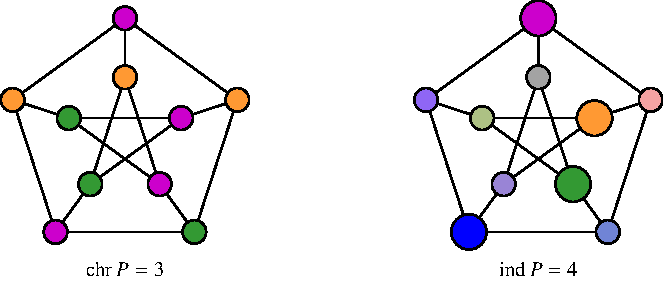
\includegraphics{chapters/70-graphen/images/petersonchrind.pdf}
\caption{Chromatische Zahl und Unabhängigkeitszahl des Peterson-Graphen.
Die chromatische Zahl ist $3$, da der Graph sich mit drei Farben einfärben
lässt (links).
Die Unabhängigkeitszahl ist $4$, die vier grösseren Knoten im rechten
Graphen sind unabhängig.
Die Farben der kleinen Knoten sind die additive Mischung der Farben
der grossen Knoten, mit denen sie verbunden sind.
\label{buch:graphen:fig:chrindpeterson}}
\end{figure}

\begin{beispiel}
Der Peterson-Graph $P$ von Abbildung~\ref{buch:graphen:fig:chrindpeterson}
hat chromatische Zahl $\operatorname{chr}P=3$ und Unabhängigkeitszahl
$\operatorname{ind}P=4$.
Die Ungleichung von Satz~\ref{buch:satz:chrind} ist erfüllt, sogar als
Ungleichung: $\operatorname{chr}P\cdot\operatorname{ind}P=3\cdot 4=12>10=n$.
\end{beispiel}

Nach Definition ist die Unabhängigkeitszahl ein Mass für die Grösse einer
unabhängigen Menge von Punkten.
Der Beweis von Satz~\ref{buch:satz:chrind} zeigt, dass man sich die
chromatische Zahl als ein Mass dafür vorstellen kann,
wieviele solche unabhängige 
Mengen in einem Graphen untergebracht werden können.

%
% Chromatische Zahl und maximaler Grad
%
\subsection{Chromatische Zahl und maximaler Grad
\label{buch:subsection:chr-und-maximaler-grad}}
Wenn kein Knoten mehr als $d$ Nachbarn hat, dann reichen
$d+1$ Farben immer, um diesen Knoten und seine Nachbarn einzufärben.
Das heisst aber noch nicht, dass dann auch $d+1$ Farben zur
Einfärbung des ganzen Graphen reichen.
Genau dies garantiert jedoch der folgende Satz.

\begin{definition}
Der {\em maximale Grad}
\(
\max_{v\in V} \deg(v)
\)
eines ungerichteten Graphen 
wird mit $d$ bezeichnet.
\index{maximaler Grad}%
\end{definition}

\begin{satz}
\label{buch:graphen:satz:chrmaxgrad}
Ist $G$ ein Graph mit maximalem Grad $d$, dann gilt 
$\operatorname{chr}G \le d+1$.
\end{satz}

\begin{proof}[Beweis]
Wir führen den Beweis mit Hilfe von vollständiger Induktion nach der
Anzahl Knoten eines Graphen.
Ein Graph mit nur einem Knoten hat keine Kanten, der maximale Grad ist
daher $0$ und $d+1=1$ Farbe reicht auch tatsächlich zur Einfärbung des
einen Knotens.

Wir nehmen jetzt an, die Behauptung sei für Graphen mit $n-1$ Knoten bereits
bewiesen, ein Graph $G'$ mit $n-1$ Knoten und maximalem Grad $d'$ erfüllt
also die Ungleichung $\operatorname{chr}G'\le d'+1$.

Wir wählen jetzt einen beliebigen Knoten $v$ des Graphen $G$ und bilden
den Graphen $G'$, der aus $G$ entsteht, indem man den Knoten $v$
entfernt: $G'=G\setminus\{v\}$.
Der maximale Grad $d'$ von $G'$ kann dabei nicht grösser werden, es ist
also $d'\le d$.
Da $G'$ genau $n-1$ Knoten hat, lässt er sich mit höchstens $d'+1\le d+1$
Farben einfärben.
Es muss jetzt also nur noch eine Farbe für den Knoten $v$ gefunden werden.
Da $d$ der maximale Grad ist, hat $v$ höchstens $d$ Nachbarn, die höchstens
$d$ verschiedene Farben haben können.
Von den $d+1$ zur Verfügung stehenden Farben bleibt also mindestens eine
übrig, mit der man den Knoten $v$ einfärben kann.
Damit ist der Induktionsschritt gelungen und somit der Satz bewiesen.
\end{proof}

Das Argument im Beweis von Satz~\ref{buch:graphen:satz:chrmaxgrad}
ist für alle Begriffe anwendbar, die sich bei der Bildung eines 
Untergraphen auf ``monotone'' Art ändern.
Die chromatische Zahl eines Untergraphen ist höchstens so gross wie die
des ganzen Graphen. 
Daher kann man eine Ungleichung für grosse Graphen schrittweise aus
entsprechenden Ungleichungen für die kleineren Teilgraphen gewinnen.
Ziel der folgenden Abschnitte ist zu zeigen, dass sich eine Grösse
mit ähnlichen Eigenschaften aus dem Eigenwertspektrum der Adjazenzmatrix
ablesen lässt.
Daraus ergibt sich dann eine bessere Abschätzung der chromatischen Zahl
eines Graphen.

%
% maximaler Eigenwert und maximaler Grad
%
\subsection{Maximaler Eigenwert von $A(G)$ und maximaler Grad
\label{buch:subsection:maximaler-eigenwert}}
Die Adjazenzmatrix $A(G)$ eines Graphen $G$  mit $n$ Knoten enthält unter
anderem auch die Information über den Grad eines Knotens.
Die Summe der Elemente einer Zeile oder einer Spalte ergibt einen Vektor,
der die Grade der Knoten als Komponenten enthält.
Ist $U$ ein $n$-dimensionaler Vektor aus lauter Einsen, dann ist
ist $A(G)U$ ein Spaltenvektor bestehend aus den Zeilensummen der Matrix 
$A(G)$ und
$U^tA(G)$ ein Zeilenvektor bestehend aus den Spaltensummen.
$A(G)U$ ist also der Vektor der Grade der Knoten.

Das Skalarprodukt von $A(G)U$ mit $U$ ist die Summe der Grade.
Somit ist
\begin{equation}
\frac{\langle A(G)U,U\rangle}{\langle U,U\rangle}
=
\frac{1}{\langle U,U\rangle}\sum_{v\in V}\deg(v)
=
\frac{1}{n}(d_1+\dots+d_n)
\label{buch:graphen:eqn:AUdavg}
\end{equation}
der {\em mittlere Grad}, der mit $\overline{d}$ bezeichnet werden soll.
Da die Kanten eines Graphen zusammen $2\cdot|E|$ Enden haben, kann
er kann auch als
\[
\overline{d}=\frac{2\cdot|E|}{|V|}
\]
berechnet werden.
\index{mittlerer Grad}%

Da $A(G)$ eine symmetrische Matrix ist, ist $A(G)$ diagonalisierbar,
die Eigenwerte sind also alle reell.
Es ist ausserdem bekannt, dass der Eigenvektor $f$ zum grössten Eigenwert
$\alpha_{\text{max}}$ von $A(G)$
den Bruch
\[
\frac{\langle A(G)f,f\rangle}{\langle f,f\rangle}
\]
für Vektoren $f\ne 0$ maximiert.
Aus~\eqref{buch:graphen:eqn:AUdavg} folgt damit, dass
\begin{equation}
\overline{d}
\le
\alpha_{\text{max}}
\label{buch:graphen:eqn:dqueramax}
\end{equation}
ist.

In Abschnitt~\ref{buch:section:positive-vektoren-und-matrizen}
des nächsten Kapitels wird die Perron-Frobenius-Theorie positiver
\index{Perron-Frobenius-Theorie}%
\index{positive Matrix}%
Matrizen vorgestellt, welche einer Reihe interessanter Aussagen
über den betragsgrössten Eigenwert und den zugehörigen Eigenvektor
macht.
Die Adjazenzmatrix ist eine nichtnegative Matrix und $\alpha_{\text{max}}$
ist der grösste Eigenwert, also genau die Grösse, auf die die
Sätze~\ref{buch:wahrscheinlichkeit:satz:perron-frobenius}
und \ref{buch:wahrscheinlichkeit:satz:perron-frobenius2}
anwendbar sind.
Dazu muss die Matrix allerdings primitiv sein, was gleichbedeutend
\index{primitive Matrix}%
ist damit, dass der Graph zusammenhängend ist.
Im folgenden soll dies daher jeweils angenommen werden.

\begin{satz}
Ist $G$ ein zusammenhängender Graph mit $n$ Knoten und maximalem Grad $d$,
dann gilt
\[
\frac1n\sum_{v\in V} \deg(v) 
=
\overline{d}
\le \alpha_{\text{max}} \le d.
\]
\end{satz}

\begin{proof}[Beweis]
Wir wissen aus \eqref{buch:graphen:eqn:dqueramax} bereits, dass
$\overline{d}\le\alpha_{\text{max}}$ gilt, es bleibt also nur noch
$\alpha_{\text{max}}\le d$ zu beweisen.

Sei $f$ der Eigenvektor zum Eigenwert $\alpha_{\text{max}}$.
Nach Satz~\label{buch:wahrscheinlichkeit:satz:perron-frobenius2}
ist $f$ ein positiver Vektor mit der Eigenschaft $A(G)f=\alpha_{\text{max}}f$.
Der Eigenvektor $f$ ist eine Funktion auf den Knoten des Graphen,
die $v$-Komponente des Vektors $f$ für einen Vertex $v\in V$ ist $f(v)$.
Die Eigenvektoreigenschaft bedeutet $(A(G)f)(v)=\alpha_{\text{max}} f(v)$.
Die Adjazenzmatrix $A(G)$ enthält in Zeile $v$ genau für diejenigen
Knoten $u\in V$ Einsen, die zu $v$ benachbart sind.
Schreiben wir $u\sim v$ für die Nachbarschaftsrelation, dann ist 
\[
(A(G)f)(v)
=
\sum_{u\sim v} f(u).
\]
Die Summe der Komponenten $A(G)f$ kann man erhalten durch Multiplikation
von $A(G)f$ mit einem Zeilenvektor $U^t$ aus lauter Einsen, also
\begin{equation}
\begin{aligned}
{\color{red}
\sum_{v\in V}}\sum_{u\sim v}f(v)
&=
{\color{red}U^t}A(G)f
=
(U^tA(G))f
=
\begin{pmatrix}d_1&d_2&\dots&d_n\end{pmatrix} f
\\
&=
\sum_{v\in V}\deg (v) f(v)
\le
\sum_{v\in V}df(v)
=
d
\sum_{v\in V}f(v).
\end{aligned}
\label{buch:graphen:eqn:sumkomp}
\end{equation}
Andererseits ist $A(G)f=\alpha_{\text{max}}f$, die linke Seite
von~\eqref{buch:graphen:eqn:sumkomp} ist daher
\begin{equation}
\sum_{v\in V}\sum_{u\sim v}f(v)
=
U^tA(G)f
=
\alpha_{\text{max}}
U^tf
=
\alpha_{\text{max}} \sum_{v\in V}f(v).
\label{buch:graphen:eqn:sumkomp2}
\end{equation}
Die Ungleichung~\eqref{buch:graphen:eqn:sumkomp}
und die Gleichung~\eqref{buch:graphen:eqn:sumkomp2} ergeben zusammen
die Ungleichung
\[
\alpha_{\text{max}} \sum_{v\in V}f(v)
\le d\sum_{v\in V}f(v)
\qquad\Rightarrow\qquad
\alpha_{\text{max}} \le d,
\]
da die Summe der Komponenten des positiven Vektors $f$ nicht verschwinden
kann.
Damit ist die Ungleichung bewiesen.
\end{proof}

%
% alpha_max eines Untergraphen
%
\subsection{$\alpha_{\text{max}}$ eines Untergraphen
\label{buch:subsection:alphamax-eines-untergraphen}}
Der grösste Eigenwert $\alpha_{\text{max}}$ ist ein potentieller 
Anwärter für eine bessere Abschätzung der chromatischen Zahl.
Bereits früher wurde bemerkt, dass dies auch bedeutet, dass man 
das Verhalten des grössten Eigenwerts bei einem Übergang zu einem
Untergraphen verstehen muss.

\begin{satz}
\label{buch:graphen:satz:amaxuntergraph}
Sei $G'$ ein echter Untergraph von $G$ mit Adjazenzmatrix $A(G')$ und
grösstem Eigenwert $\alpha_{\text{max}}'=\varrho(A(G'))$, dann ist
$\alpha_{\text{max}}' \le \alpha_{\text{max}}$.
\end{satz}

\begin{proof}[Beweis]
Sei $f'$ der positive Eigenvektor zum Eigenwert $\alpha_{\text{max}}'$
der Matrix $A(G')$.
$f'$ ist definiert auf der Menge $V'$ der Knoten von $G'$.
Aus $f'$ lässt sich ein Vektor $g$ mit den Werten
\[
g(v)
=
\begin{cases}
f'(v)&\qquad v\in V'\\
    0&\qquad\text{sonst}
\end{cases}
\]
konstruieren, der auf ganz $V$ definiert ist.

Die Vektoren $f'$ und $g$ haben auf $V'$ die gleichen Komponenten, also ist auch
$\langle f',f'\rangle = \langle g,g\rangle$.
Die Matrixelemente von $A(G')$ und $A(G)$ auf gemeinsamen Knoten $u,v\in V'$ 
erfüllen $A(G')_{uv}\le A(G)_{uv}$, da jede Kante von $G'$ auch in $G$ ist.
Daher gilt
\[
\langle A(G')f',f'\rangle
\le
\langle A(G)g,g\rangle,
\]
woraus sich die Ungleichung
\[
\alpha_{\text{max}}'
=
\frac{\langle A(G')f',f'\rangle}{\langle f',f'\rangle}
=
\frac{\langle A(G)g,g\rangle}{\langle g,g\rangle}
\le
\alpha_{\text{max}}
\]
ergibt, da $\alpha_{\text{max}}$ das Maximum von
$\langle A(G)h,h\rangle/\langle h,h\rangle$ für alle Vektoren $h\ne 0$ ist.
\end{proof}

%
% Der Satz von Wilf
%
\subsection{Chromatische Zahl und $\alpha_{\text{max}}$: Der Satz von Wilf
\label{buch:subsection:chr-und-alpha-max}}
\index{Satz von Wilf}%
\index{Wilf, Satz von}%
Die in Satz~\ref{buch:graphen:satz:amaxuntergraph} beschriebene
Eigenschaft von $\alpha_{\text{max}}$ beim Übergang zu einem Untergraphen
ermöglich jetzt, eine besser Abschätzung für die chromatische Zahl
zu finden.

\begin{satz}[Wilf]
\label{buch:graphen:satz:wilf}
Sie $G$ ein zusammenhängder Graph und $\alpha_{\text{max}}$ der grösste
Eigenwert seiner Adjazenzmatrix. Dann gilt
\[
\operatorname{chr}G\le \alpha_{\text{max}}+1.
\]
\end{satz}

\begin{proof}[Beweis]
Wie der Satz~\ref{buch:graphen:satz:chrmaxgrad} kann auch der Satz von Wilf
mit Hilfe von vollständiger Induktion über die Anzahl $n$ der Knoten
bewiesen werden.

Ein Graph mit nur einem Knoten hat die $0$-Matrix als Adjazenzmatrix,
der maximale Eigenwert ist $\alpha_{\text{max}}=0$, und tatsächlich reicht
$\alpha_{\text{max}}+1=1$ Farbe, um den einen Knoten einzufärben.
Dies ist die Induktionsverankerung.

Im Sinne der Induktionsannahme 
nehmen wir jetzt an, der Satz sei für Graphen mit $n-1$ Knoten bereits
beweisen.
Wir müssen dann zeigen, dass der Satz dann auch für Graphen mit $n$ Knoten
gilt.

Sei $v\in V$ ein Knoten minimalen Grades und $G'=G\setminus\{v\}$ der
Untergraph, der entsteht, wenn der Knoten $v$ entfernt wird.
Da $G'$ genau $n-1$ Knoten hat, gilt der Satz von Wilf für $G'$
und daher kann $G'$ mit höchstens
\[
\operatorname{chr}G' \le 1 + \alpha_{\text{max}}'
\]
Farben eingefärbt werden.
Nach Satz~\ref{buch:graphen:satz:amaxuntergraph} ist
$\alpha_{\text{max}}'\le \alpha_{\text{max}}$,
Also kann $G'$ mit höchstens $\alpha_{\text{max}}+1$ Farben eingefärbt werden.

Da $v$ ein Knoten minimalen Grades ist, ist sein Grad
$d(v)\le \overline{d}\le \alpha_{\text{max}}$.
Die Nachbarn von $v$ haben also hächstens $\alpha_{\text{max}}$ verschiedene
Farben, mit einer weiteren Farbe lässt sich also auch $G$ einfärben.
Daraus folgt $\operatorname{chr}G\le \alpha_{\text{max}}+1$.
\end{proof}

\begin{figure}
\centering
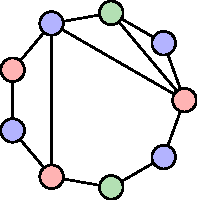
\includegraphics{chapters/70-graphen/images/nine.pdf}
\caption{Beispiel für einen Graphen, für den der
Satz~\ref{buch:graphen:satz:wilf} von Wilf die bessere
Abschätzung für die chromatische Zahl eines Graphen gibt als der
maximale Grad.
\label{buch:graphen:fig:wilfexample}}
\end{figure}

\begin{beispiel}
Der Graph in Abbildung~\ref{buch:graphen:fig:wilfexample} hat 12 Kanten und 9
Knoten, daher ist $\overline{d}\le \frac{24}{9}$.
Der maximale Grad ist $4$ und durch explizite Rechnung mit Hilfe zum Beispiel
von Octave ergibt, dass $\alpha_{\text{max}}\approx 2.9565$.
Aus dem Satz von Wilf folgt, dass
$\operatorname{chr}G\le \alpha_{\text{max}}+1$, und daraus ergibt sich
$\operatorname{chr}G\le 3$.
Tatsächlich ist die chromatische Zahl $\operatorname{chr}G=3$, da 
der Graph mindestens ein Dreieck enthält.
Der maximale Grad ist 4, somit gibt der
Satz~\ref{buch:graphen:satz:chrmaxgrad}
die Schranke 
$\operatorname{chr}G\le 4+1=5$
für die chromatische Zahl.
Der Satz von Wilf ist also eine wesentliche Verbesserung, er liefert in
diesem Fall den exakten Wert der chromatischen Zahl.
\end{beispiel}




%
% waerme.tex
%
% (c) 2020 Prof Dr Andreas Müller, Hochschule Rapperswil
%
\section{Wärmeleitung auf einem Graphen
\label{buch:section:waermeleitung-auf-einem-graphen}}
Die Vektoren, auf denen die Laplace-Matrix operiert, können betrachtet
werden als Funktionen, die jedem Knoten einen Wert zuordnen.
Eine mögliche physikalische Interpretation davon ist die Temperaturverteilung
auf dem Graphen.
Die Kanten zwischen den Knoten erlauben der Wärmeenergie, von einem Knoten
zu einem anderen zu fliessen.
Je grösser die Temperaturdifferenz zwischen zwei Knoten ist, desto
grösser ist der Wärmefluss und desto schneller ändert sich die Temperatur
der beteiligten Knoten.
Die zeitliche Änderung der Temperatur $T_i$ im Knoten $i$ ist proportional
\[
\frac{dT_i}{dt}
=
\sum_{\text{$j$ Nachbar von $i$}} \kappa (T_j-T_i)
=
-
\kappa
\biggl(
d_iT_i
-
\sum_{\text{$j$ Nachbar von $i$}} T_j
\biggr)
\]
Der Term auf der rechten Seite ist genau die Wirkung der 
Laplace-Matrix auf dem Vektor $T$ der Temperaturen:
\begin{equation}
\frac{dT}{dt}
=
-\kappa L T.
\label{buch:graphen:eqn:waermeleitung}
\end{equation}
Der Wärmefluss, der durch die
Wärmeleitungsgleichung~\eqref{buch:graphen:eqn:waermeleitung} beschrieben
wird, codiert ebenfalls wesentliche Informationen über den Graphen.
Je mehr Kanten es zwischen verschiedenen Teilen eines Graphen gibt,
desto schneller findet der Wärmeaustausch zwischen diesen Teilen
statt.
Die Lösungen der Wärmeleitungsgleichung liefern also Informationen 
über den Graphen.

\subsection{Eigenwerte und Eigenvektoren
\label{buch:subsection:ein-zyklischer-graph}}
Die Wärmeleitungsgleichung~\eqref{buch:graphen:eqn:waermeleitung} 
ist eine lineare Differentialgleichung mit konstanten Koeffizienten,
die mit der Matrixexponentialfunktion gelöst werden.
Die Lösung ist
\[
f(t) = e^{-\kappa Lt}f(0).
\]

Die Berechnung der Lösung mit der Matrixexponentialreihe ist ziemlich
ineffizient, da grosse Matrizenprodukte berechnet werden müssen.
Da die Matrix $L$ symmetrisch ist, gibt es eine Basis aus 
orthonormierten Eigenvektoren und die Eigenwerte sind reell.
Wir bezeichnen die Eigenvektoren mit $f_1,\dots,f_n$  und die
zugehörigen Eigenwerte mit $\lambda_i$.
Die Funktion $f_i(t)= e^{-\kappa\lambda_it}f_i$ ist dann eine Lösung
der Wärmeleitungsgleichung, denn die beiden Seiten
\begin{align*}
\frac{d}{dt}f_i(t)
&=
-\kappa\lambda_ie^{-\kappa\lambda_it}f_i
=
-\kappa\lambda_i f_i(t)
\\
-\kappa Lf_i(t)
&=
-\kappa e^{-\kappa\lambda_it} Lf_i
=
-\kappa e^{-\kappa\lambda_it} \lambda_i f_i
=
-\kappa \lambda_i f_i(t)
\end{align*}
von \eqref{buch:graphen:eqn:waermeleitung} stimmen überein.

Eine Lösung der Wärmeleitungsgleichung zu einer beliebigen
Anfangstemperaturverteilung $f$ kann durch Linearkombination aus 
den Lösungen $f_i(t)$ zusammengesetzt werden.
Dazu ist nötig, $f$ aus den Vektoren $f_i$ linear zu kombinieren.
Da aber die $f_i$ orthonormiert sind, ist dies besonders einfach,
die Koeffizienten sind die Skalarprodukte mit den Eigenvektoren:
\[
f=\sum_{i=1}^n \langle f_i,f\rangle f_i.
\]
Daraus kann man die allgmeine Lösungsformel
\begin{equation}
f(t)
=
\sum_{i=1}^n \langle f_i,f\rangle f_i(t)
=
\sum_{i=1}^n \langle f_i,f\rangle e^{-\kappa\lambda_i t}f_i
\label{buch:graphen:eqn:eigloesung}
\end{equation}
ableiten.

\subsection{Beispiel: Ein zyklischer Graph}
\begin{figure}
\centering
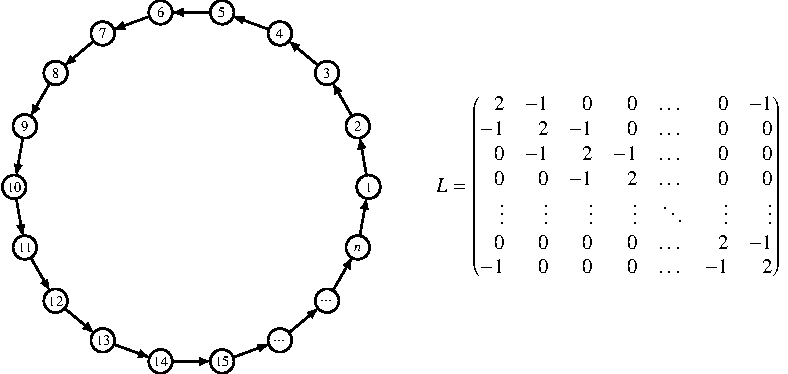
\includegraphics{chapters/70-graphen/images/kreis.pdf}
\caption{Beispiel Graph zur Illustration der verschiedenen Basen auf einem
Graphen.
\label{buch:graphen:fig:kreis}}
\end{figure}
Wir illustrieren die im folgenden entwickelte Theorie an dem Beispielgraphen
von Abbildung~\ref{buch:graphen:fig:kreis}.
Besonders interessant sind die folgenden Funktionen:
\[
\left.
\begin{aligned}
s_m(k)
&=
\sin\frac{2\pi mk}{n}
\\
c_m(k)
&=
\cos\frac{2\pi mk}{n}
\end{aligned}
\;
\right\}
\quad
\Rightarrow
\quad
e_m(k)
=
e^{2\pi imk/n}
=
c_m(k) + is_m(k).
\]
Das Skalarprodukt dieser Funktionen ist
\[
\langle e_m, e_{m'}\rangle
=
\frac1n
\sum_{k=1}^n
\overline{e^{2\pi i km/n}}
e^{2\pi ikm'/n}
=
\frac1n
\sum_{k=1}^n
e^{\frac{2\pi i}{n}(m'-m)k}
=
\delta_{mm'}
\]
Die Funktionen bilden daher eine Orthonormalbasis des Raums der
Funktionen auf $G$.
Wegen $\overline{e_m} = e_{-m}$ folgt, dass für gerade $n$
die Funktionen
\[
c_0, c_1,s_1,c_2,s_2,\dots c_{\frac{n}2-1},c_{\frac{n}2-1},c_{\frac{n}2}
\]
eine orthonormierte Basis.


Die Laplace-Matrix kann mit der folgenden Definition zu einer linearen
Abbildung auf Funktionen auf dem Graphen gemacht werden.
Sei $f\colon V\to \mathbb{R}$ und $L$ die Laplace-Matrix mit
Matrixelementen $l_{vv'}$ wobei $v,v'\in V$ ist.
Dann definieren wir die Funktion $Lf$ durch
\[
(Lf)(v)
=
\sum_{v'\in V} l_{vv'}f(v').
\]

\subsection{Standardbasis und Eigenbasis
\label{buch:subsection:standardbasis-und-eigenbasis}}
Die einfachste Basis, aus der siche Funktionen auf dem Graphen linear
kombinieren lassen, ist die Standardbasis.
Sie hat für jeden Knoten $v$ des Graphen eine Basisfunktion mit den Werten
\[
e_v\colon V\to\mathbb R:v'\mapsto \begin{cases}
1\qquad&v=v'\\
0\qquad&\text{sonst.}
\end{cases}
\]



%
% wavelets.tex -- Wavelets auf Graphen
%
% (c) 2020 Prof Dr Andreas Müller, Hochschule Rapperswil
%
\section{Wavelets auf Graphen
\label{buch:section:wavelets-auf-graphen}}
\rhead{Wavelets auf Graphen}


